\chapter{Elektronik und Sicherheit}
\label{sec:elektronikUndSicherheit}

\section{Abstract}
\label{sec:abstract}

Because of the electronic part, the horse exerciser should be able to rotate. 
The actuator of the engine is realised by a frequency converter, which gets the signals from the GPIO-Pins on the Raspberry-Pi.
How fast the horse exerciser will move, depends on the commands, that he recives over the Ethernet from the webserver.
The horses will get a refreshment on hot sommer days by the use of the electric water valve.
Due to the fact that the system will be used to exercise animals, one of the most important points is the safety of the horses.

\section{Zusammenfassung}
\label{sec:zusammenfassung}

Der Elektronikteil soll dazu dienen, die Pferdeführanlage in den gewünschten Geschwindigkeiten zu drehen, welche über die App für die Pferde gewählt wurden. 
Die Ansteuerung des Motors kann mit einem Frequenzumrichter realisiert werden, 
welcher die Signale von einem gewünschten Kommunikationssystem bekommt.
Des weiteren bekommt die Steuereinheit über Ethernet die Befehle, wie schnell sich die Anlage drehen darf und wie lange. 
Mittels eines elektrischen Wasserventils, wird den Pferden an heißen Sommertagen eine Erfrischung ermöglicht. 
Da mit der Anlage Tiere trainiert werden sollen, ist der wichtigste Nebenpunkt die Sicherheit der Pferde und natürlich von der Anlage selbst.
%%%
\newpage
%%%

\section{Aufgabenbereich}
\label{sec:aufgabenbereich}

Mein Aufgabenbereich bei der Diplomarbeit ,,Pferdeführanlage“, ist die Planung für die Elektronik. Wie bereits bei der Hauptaufgabenstellung (1.1.?) erwähnt, 
soll sich die Anlage mit verschiedenen Geschwindigkeiten und Variationen drehen.  Neben der Steuerung der Anlage, muss man auch auf die Sicherheit der Pferde achten.
\\
\\
Mein Aufgabenbereich bei der Diplomarbeit sind:

\begin{itemize}
\item Auswahl des Motors
\item Ansteuerung des Motors
\item Auswahl der Sensoren
\item Auswahl eines Ventils
\item Kommunikation zu Web-Server
\item Schutz des Pferdes und der Anlage
\end{itemize}
%%%%
\newpage
%%%%
\section{Vorarbeit}
\label{sec:vorarbeit}

Um die Suche ein wenig einzugrenzen, wurden persönliche Vorgaben festgelegt.
Diese Vorgaben konnten durch Erfahrung oder Gespräche erstellt werden.

\subsection{Motor}
\label{sec:motor}

Prinzipiell könnte man die Anlage auch rein mechanisch Ansteuern. Mit der Hilfe von Wind, Wasser oder Öl, diese sind aber wetter- und ortsbedingt, im letzten Fall noch eine zusätzliche Umweltbelastung. Da in Mitteleuropa fast jeder Haushalt eine Stromanbindung hat, wurde der Fokus auf die Elektromotoren gerichtet.

\subsection{Ansteuerung Elektromotor}
\label{sec:ansteuerungElektromotor}

Um einen Motor gezielt und einfach steuern zu können, wird in den meisten Fällen auf einen Frequenzumrichter zurückgegriffen. Alternative dazu wäre ein Motorstarter. Mit diesen lassen sich aber nicht so einfach die Geschwindigkeiten steuern.

\subsection{Wasserversorgung Sprühregen}
\label{sec:wasserversorgungSpruehregen}

Für die Wasserversorgung wird ein 1 Zoll Wasseranschluss benötigt. Dieser ist normaler Weise bei jedem Haus vorhanden. 
Sollte dies nicht der Fall sein, ist es auch möglich eine Zuleitung mit geringeren Durchmesser nehmen.

\subsection{Verarbeitung der Daten}
\label{sec:verarbeitungDerDaten}

Da sowohl das Senden von elektrischen Signalen, als auch die Kommunikation über ein Netzwerk realisiert werden soll, sollte ein System verwendet werden, welches beides direkt verarbeiten kann. 

\subsection{Pferde Sicherheit}
\label{sec:pferdeSicherheit}

Man darf bei der Anlage nicht auf die allgemeine Sicherheit vergessen. Überall können Fehler auftreten. Bei einem Fehler muss man wissen, wie man die Pferde, Menschen und auch die Anlage schützt. Dazu gehören allgemeine Fehler, NOT-AUS und NOT-STOPP.
%%%%
\newpage
%%%%

\section{Antriebstechnik Grundlagen}
\label{sec:antriebstechnikGrundlagen}

\subsection{Aufbau}
\label{sec:aufbau}
\begin{figure}[!ht]
\begin{center}
	\caption{Aufbau Antriebstechnik}
	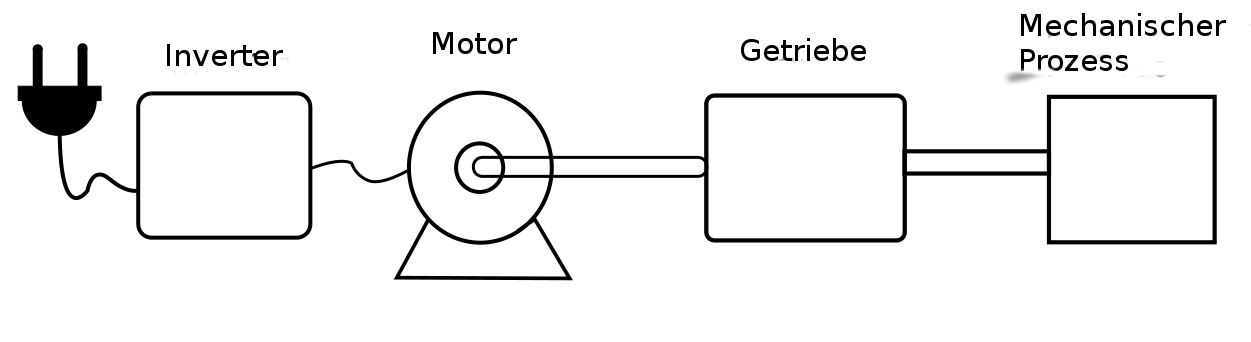
\includegraphics[width=1\textwidth]{AntriebstechnikAufbau}
\end{center}
\end{figure}

Der Inverter wandelt die vorhandene elektrische Energie in die gewünschte elektrische Ausgangsgröße um. 
Diese wird so gewählt, dass der Motor direkt damit betrieben werden kann. Dieser kann durch der Welle den gewünschten mechanischen Prozess betreiben.  Falls man die Drehzahl nicht elektrisch verändern will, benötigt man zusätzlich ein Getriebe. Das Getriebe kann aber auch nur als Verbindung dienen und mittels Keilriemen oder ähnlichem realisiert werden.

Daraus ergibt sich folgender Ablauf wie aus der Abbildung oben ersichtlich:
$Versorgungsspannung \rightarrow Inverter \rightarrow Motor \rightarrow (Getriebe) \rightarrow Mechanischer Prozess$

\subsection{Anforderungen}
\label{sec:anforderungen}

Ein Antriebssystem sollte gewissen Anforderungen entsprechen, um vermarktbar zu sein. Folgende Auflistung zeigt die wichtigsten Punkte:

\begin{itemize}
\item{Stabile Steuerung der Geschwindigkeit}
\item{Verbundene Mechanik mit hoher Genauigkeit ansteuern}
\item{Stabile Kraftanwendung}
\end{itemize}

%%%
\newpage
%%%

\section{Elektromotor}
\label{sec:elektromotor}

\subsection{Grundprinzip}
\label{sec:grundprinzip}

Die Kraft, welche den Elektromotor in Bewegung versetzt, nennt sich Lorentzkraft.
Befindet sich ein stromdurchflossener elektrischer Leiter in einem Magnetfeld, so wirkt auf diesen Leiter eine Kraft.
Die Wirkungsrichtung hängt von der Stromflussrichtung im Leiter ab. 
Um sich die Vorstellung zu erleichtern, wird in den meisten Fällen die "Linke-Hand-Regel" verwendet.

\begin{figure}[!ht]
\begin{center}
	\caption{Link-Hand-Regel}
	\includegraphics[width=0.35\textwidth]{LinkehandRegel}
\end{center}
\end{figure}

Die Lorentzkraft wird mit folgender Formel festgelegt:

\begin{equation}
\label{eq:1}
 F = B * I * l
\end{equation}
\begin{center}
F= Lorentzkraft, B= magnetische Flussdichte, \\ I = Stromstärke, l = Länge des Leiters im Magnetfeld
\end{center}

Aus der Formel lässt sich entnehmen, dass die Lorentzkraft von der magnetischen Flussdichte, Stromstärke und Länge des Leiters abhängt.

Diese Kraft erzeugt bei einer Lagerung von der Spule, ein Moment, welches das gewünschte System drehen lässt.

\subsection{Motorarten}
\label{sec:motorarten}

Es gibt viele verschiedene Motorarten und Typen. Um eine kleine Übersicht zu ermöglichen werden nachfolgend die wichtigsten Grundmotore aufgelistet und ein wenig näher beschrieben.

\subsubsection{Gleichstrommotor}
\label{sec:gleichstrommotor}

Der Rotor wird gelagert und mehrfach mit Draht umwickelt. Der Rotor bekommt über Kohlebürsten am Kollektor eine Stromübertragung. Daraufhin bekommt der Rotor erneuten Schwung mit.
Wenn der Motor größer sein muss, kann der Stator in mehrere Pole aufgeteilt werden. Der Stromfluss wird dadurch stabiler.

\begin{figure}[!ht]
\begin{center}
	\caption{Aufbau Gleichstrommaschine}
	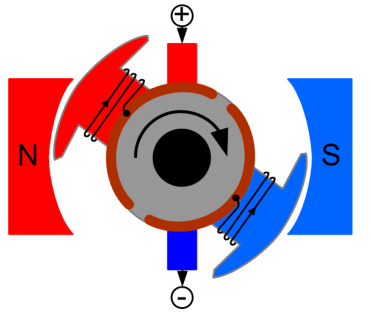
\includegraphics[width=0.3\textwidth]{Gleichstommaschine}
\end{center}
\end{figure}

Das Foto zeigt den einfachen Aufbau von einer Gleichstrommaschine. Er ist bei einfachen Anwendungen sehr beliebt, da sich die Drehzahl durch Veränderung der Versorgungsspannung ändert.\newline

\textbf{Anwendungsbereiche:}

\begin{itemize}
	\item{Scheibenwischermotoren}
	\item{Fensterheber}
	\item{Handstaubsauger}
\end{itemize}

\subsubsection{Drehstrommotor}
\label{sec:drehstrom}

Drehmaschinen arbeiten durch die Variation im Statorfeld. Der Rotor wird auch hier durch einen Magneten realisiert. Der Rotor versucht sich immer bei den entsprechenden Magnetpol zu bleiben. Die Spannungen beim Drehstrom sind um 120 versetzt. Deshalb variieren die magnetischen Pole regelmäßig. Aus diesem Grund beginnt der Rotor zu drehen.

\begin{figure}[!ht]
\begin{center}
	\caption{Aufbau Drehfeldmaschine}
	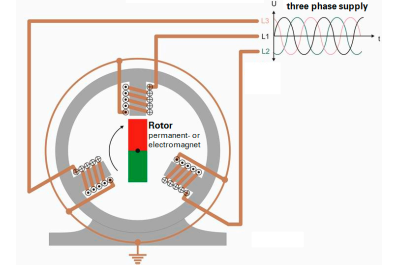
\includegraphics[width=0.5\textwidth]{Drehstrommotor}
\end{center}
\end{figure}

Bei den Drehfeldmaschinen gibt es zwei verschiedene Aufbauarten: Asynchron- und Synchronmaschine.

\subsubsection{Asynchronmotor}
\label{sec:asynchronmotor}

Ein Asynchronmotor hat einen Kurzschlussläufer.
Bei einem Kurzschlussläufer werden die Leiter, wie der Name erraten lässt, im Rotor kurzgeschlossen. Wenn der Rotor dem elektrischen Feld des Stators ausgesetzt wird, bekommen die kurzgeschlossenen Leiter eine Spannung, die einen Stromfluss verursachen. Im Rotor befindet sich jetzt ebenfalls ein eigenes Magnetfeld. Nun wirken die Magnetfelder entgegen und somit verursachen die Kräfte eine Drehbewegung. 

\textbf{Anwendungsbereiche:}

\begin{itemize}
	\item{Pumpen}
	\item{Kompressoren}
	\item{Ventilatoren}
\end{itemize}

\subsubsection{Synchronmotor}
\label{sec:synchronmotor}

Bei einer Synchronmaschine ist der Rotor entweder als Permanent- oder Elektromagnet realisiert. Dadurch hat der Rotor bereits ein eigenständiges Magnetfeld. Der Rotor kann sich deshalb selbständig auf das Magnetfeld im Stator ausrichten. Der Rotor kann nun, je nach Änderung des Magnetfeldes im Stator, direkt mitlaufen. 

\textbf{Anwendungsbereiche:}

\begin{itemize}
	\item{Roboter}
	\item{CNC-Anwendungen}
	\item{Positionierantriebe}
\end{itemize}



\subsection{Motorauswahl}
\label{sec:motorauswahl}

\begin{figure}[!ht]
\begin{center}
	\caption{Tabelle Übersicht Elektromotor}
	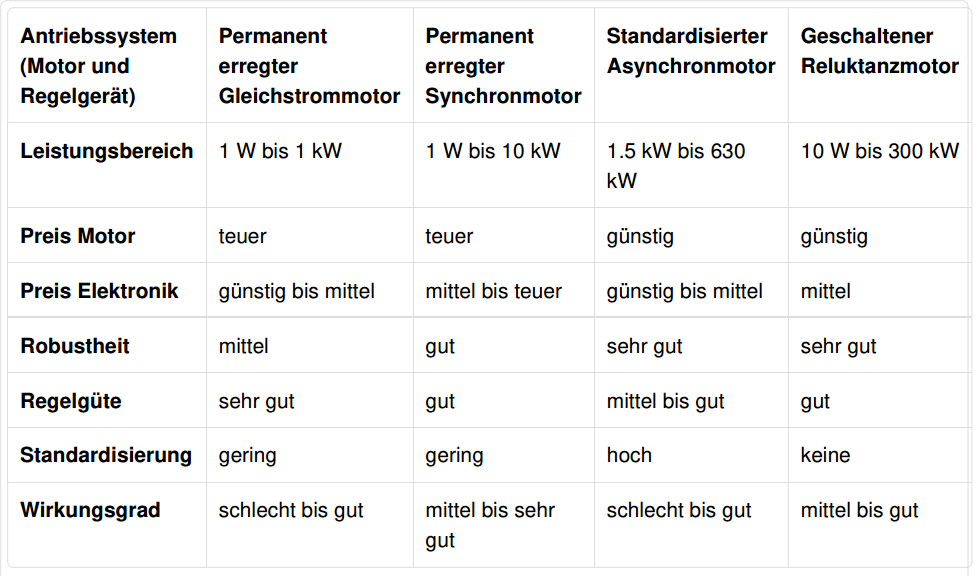
\includegraphics[width=1\textwidth]{TabelleMotor}
\end{center}
\end{figure}

Die Tabelle gibt einen Überblick, in welchen Bereich man seinen gesuchten Motor finden kann. 
Um weiter den gewünschten Motor auswählen zu können, benötigt man die Daten, was überhaupt bewegt werden soll und wie. 

\subsubsection{Festlegung des Motors}
\label{sec:festlegungDesMotors}

Aufgrund der oben angeführten Tabelle, ging der Fokus auf den Bereich der Asynchronmotoren. Man kann sie sehr oft am Markt in verschiedensten Ausführungen finden. Dadurch ist auch ein sehr gutes Preis/Leistung-Verhältnis gegeben. 
\\
Folgende Auflistung zeigt noch einmal die konkreten Vor- und Nachteile von einem Asynchronmotor:


\textbf{Vorteile:}

\begin{itemize}
	\item{Günstig}
	\item{Hohe Standardisierung}
	\item{Robust und Wartungsarm}
\end{itemize}

\textbf{Nachteile:}

\begin{itemize}
	\item{Etwas schwieriger zu Regeln}
\end{itemize}

\subsubsection{Motoranforderungen}
\label{sec:motoranforderungen}

Der Laufradius der Pferdeführanlage beträgt 9,5 Meter. Bei diesem Radius kann man die Pferde nicht galoppieren lassen. 
Für eine geeignete Geschwindigkeit wurde ein realistischer Wert gefunden. %equivetinfo.de/html/eckdaten_pferd.html 5.1.18 16:35%
Unsere Konstruktion dreht sich, wie bereits im Kapitel ?.?.? erwähnt, mit nur 5,3 min\textsuperscript{-1}. 

Vom Konstrukteur der Anlage bekomme ich zusätzlich folgende Angaben, die der Antrieb erfüllen soll:
\\

\begin{itemize}
	\item{Trägheitmoment I = 30273,53 kgm\textsuperscript{2}}
	\item{Beschleunigung $\alpha$ = 0,0947 1/s\textsuperscript{2}}
	\item{Geschwindigkeit $\omega$= 0,5 1/s}
\end{itemize}

Durch diese Angaben lässt sich ein geeigneter Motor unter folgender Berechnung finden:
\\
\textit{M\textsubscript{A} = Drehmoment der Anlage} \newline
\textit{P\textsubscript{A} = Leistung der Anlage} \newline
\textit{M\textsubscript{M} = Drehmoment des Motors} \newline
\textit{P\textsubscript{M} = Leistung des Motors} \newline
\textit{$\eta$\textsubscript{GM} = Wirkungsgrad von Motor und Übersetzung = 0,81}


\begin{center}
\begin{equation}
  \label{eq:2}
	M_{A} = I * \alpha = 30273,53kgm^2 * 0,0947 \dfrac{1}{s^2} = 2866,9 Nm
\end{equation} 
\end{center}


 
\begin{center}
\begin{equation}
  \label{eq:3}
	P_{A} = M_{A} * \omega = 2866,9 Nm * 0,5 \dfrac{1}{s} = 1433,45W
\end{equation} 
\end{center}

Beide Formeln welche oberhalb verwendet wurden, sind grundlegende Formeln in der Mechanik. Daraus konnte das benötigte Drehmoment und die benötigte Leistung der Anlage berechnet werden. Systeme haben in der Realität aber Verluste. Diese werden mit dem Wirkungsgrad festgelegt. Wenn man diesen vernachlässigt, könnte der gesuchte Antrieb überfordert sein und dadurch die Anlage nicht bewegen. Dadurch muss man folgende Rechnung durchführen:

\begin{center}
\begin{equation}
  \label{eq:4}
	\eta_{GM}= \frac{P_{A}}{P_{M}} \rightarrow P_{M} = \frac{P_{A}}{\eta_{GM}} = \frac{1433,45W}{0,81} = 1769,69W
\end{equation} 
\end{center}




\subsubsection{Auswahlverfahren}
\label{sec:auswahlverfahren}

Aufgrund der Anforderungen fiel die Entscheidung auf die Asynchronmotoren. Da die Anlage mit sehr geringer Drehzahl fährt, besteht die Möglichkeit ein externes Getriebe oder direkt auf einen Getriebemotor zurückzugreifen. 
Am Häufigsten findet man bei uns eine 230V Steckdose. Drehstromsteckdosen sind meist nur an den Orten platziert, wo sie von Anfang an benötigt werden. Um den Besitzer keine Umbauarbeiten aufzulegen liegt der Fokus bei einen 230V Anschluss. Wenn man den Motor mit Drehstrom betreiben will, ändert sich der Nennstrom des Motors. Ansonsten funktioniert er gleich.

Nun musste ein Asynchronmotor mit einer Leistung von mindestens 1770 Watt gefunden werden.


Bei der Suche nach einen geeigneten Motor kamen folgende 2 in die engere Auswahl:

\begin{figure}[!ht]
\begin{minipage}[t]{0.45\textwidth}
\framebox[\textwidth]{Motor 1}
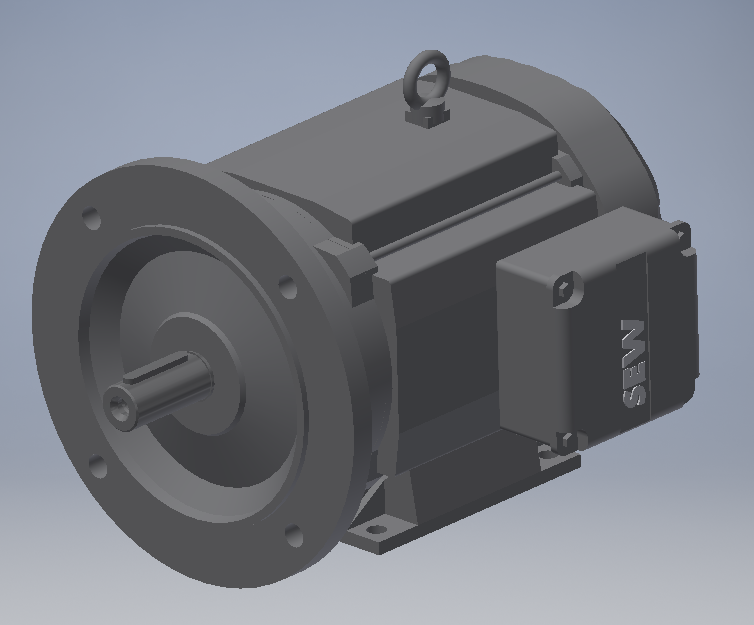
\includegraphics[width=\textwidth]{SEWMotor}
\caption{SEW-Motor}

\begin{itemize}
	\item{Motorspannung: 230/400V}
	\item{Motorstrom: 8,3/4,75A}
	\item{Motorleistung: 2,2 kW}
	\item{Drehzahl: 1450 min\textsuperscript{-1}}
	\item{Flanschdurchmesser: 250mm}
	\item{Effizienzklasse: IE3}
	\item{Motorschutzart: IP55}
	\item{Nettogewicht: 26,9kg}
\end{itemize}

\end{minipage}
\hspace{0.1\textwidth}
\begin{minipage}[t]{0.45\textwidth}
\framebox[\textwidth]{Motor 2}

%\vspace{-\ht\strutbox}
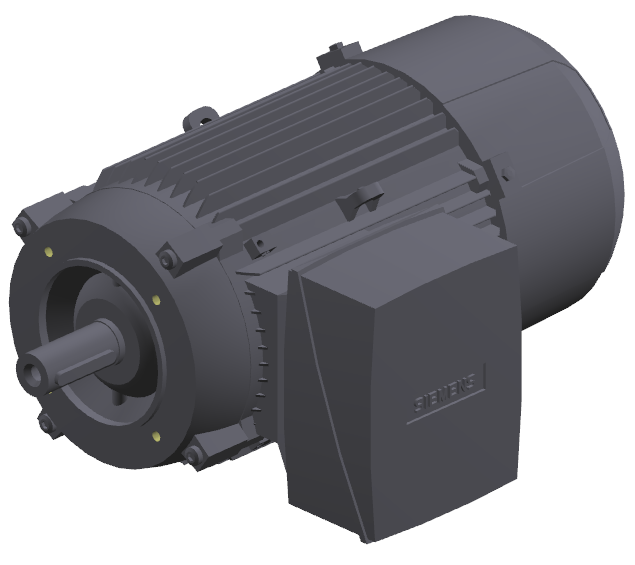
\includegraphics[width=0.93\textwidth]{SiemensMotor}
\caption{Siemens-Motor}

\begin{itemize}
	\item{Motorspannung: 230/400V}
	\item{Motorstrom: 6,6/3,75A}
	\item{Motorleistung: 1,77 kW}
	\item{Drehzahl: 1465 min\textsuperscript{-1}}
	\item{Flanschdurchmesser: -}
	\item{Effizienzklasse: IE3}
	\item{Motorschutzart: IP56}
	\item{Nettogewicht: 40kg}
\end{itemize}

\end{minipage}
\end{figure}

Für den weiteren Verlauf wurde der Motor von den Unternehmen SEW verwendet.

Da der Motor eine Drehzahl von umgerechnet 24,16s\textsuperscript{-1} hat, muss man die Drehzahl reduzieren. Um dies zu ermöglichen muss man eine Übersetzung ermöglichen. Dafür gibt es mehrere Varianten. Nachfolgend werden zwei Varianten aufgelistet:

\begin{itemize}
	\item{Motor mit externen Getriebe}
	\item{Getriebemotor}
\end{itemize}

Bei einem Getriebemotor wird das Getriebe direkt vom Hersteller auf den Motor ausgelegt. Bei einen externen Getriebe muss man zusätzlich darauf achten, das der Motor mit dem Getriebe verbunden werden kann beziehungsweise darf. Um den zusätzlichen Arbeitsaufwand gering zu halten und bei Komplikationen auf den jeweiligen Hersteller zurückgreifen kann, wird für die Pferdeführanlage ein Getriebemotor verwendet.

\subsubsection{Getriebemotor}
\label{sec:getriebemotor}

Ein Getriebemotor  besteht aus einem Motor und einem Getriebe, welche direkt in einer gemeinsamen Einheit miteinander verbunden sind. Das Getriebe soll sowohl Drehzahl als auch Drehmoment des Motors wandeln. Diese Wandlung kann mittels Drehzahlverhältnis ermittelt werden. Bei Getriebemotoren muss man das Drehmoment von Motor und Getriebe beachten. Primär gilt die Last die auf das Getriebe wirkt. 
Wie auch bei allen anderen Motoren gibt es auch bei den Getriebemotoren viele weitere Modelle. Zum Beispiel Servo-Getriebemotore und Verstellbare-Getriebemotore.

Für unsere Anlage wurde folgender Getriebemotor gefunden:

\begin{figure}[!ht]
\begin{center}
	\caption{SEW-Getriebemotor}
	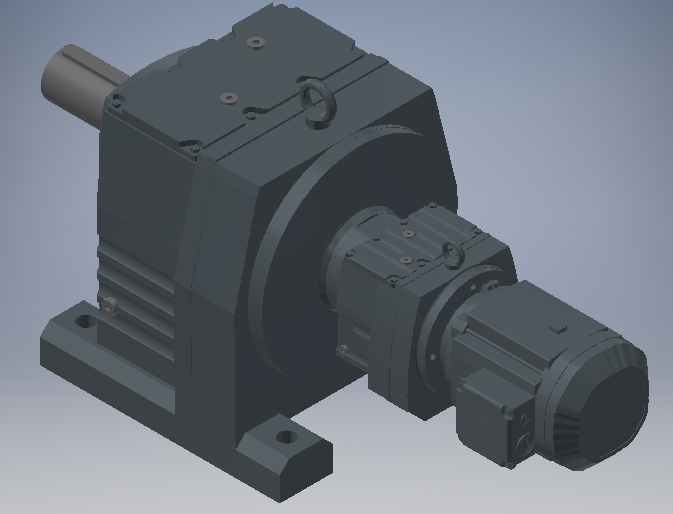
\includegraphics[width=0.5\textwidth]{SEWGetriebemotor}
\end{center}
\end{figure}

Der Getriebemotor hat folgende Daten:

\begin{itemize}
	\item{Motorspannung: 230/400V}
	\item{Motorstrom: 8,3/4,75A}
	\item{Motorleistung: 2,2 kW}
	\item{Motordrehzahl: 1450 min\textsuperscript{-1}}
	\item{Abtriebsdrehzahl: 6,5 min\textsuperscript{-1}}
	\item{Abtriebsdrehmoment: 2980 Nm}
	\item{Übersetzung i: 223,00}
	\item{Effizienzklasse: IE3}
	\item{Motorschutzart: IP56}
	\item{Nettogewicht: 341kg}
\end{itemize}

Wenn man diesen Motor mit den Motoranforderungen vergleicht, werden folgende Anforderungen, durch den Getriebemotor, erfüllt:

\begin{itemize}
	\item{Mindestens Drehmoment: 2866,9 Nm; Tatsächliches Drehmoment: 2980 Nm}
	\item{Mindestleistung: 1769,69W; Tatsächliche Leistung: 2200W}
\end{itemize}

Das einzige was noch nicht ganz passt ist die Abtriebsdrehzahl bei 50 Hz. Um auf die gewünschte Drehzahl zu kommen gibt es zwei Varianten. Entweder man sorgt über Riemenscheiben für die restliche Übersetzung oder man konfiguriert den Frequenzumrichter mit einer maximalen Frequenz, die auf den Motor wirken darf. \\

Da man sowieso die Ausgangswelle mit der Anlage verbinden muss, werden auf Riemenscheiben verwendet.

Um die jeweiligen Durchmesser der Riemenscheibe zu ermitteln, muss man das benötigte Übersetzungsverhältnis ermitteln.

\begin{center}
\begin{equation}
  \label{eq:5}
	i=  \frac{n_{Antrieb}}{n_{Abtrieb}} \rightarrow i = \frac{6,5 min\textsuperscript{-1}}{4,77 min\textsuperscript{-1}} = 1,362
\end{equation} 
\end{center}

Um den gewünschten Durchmesser zu finden muss man einen Durchmesser annehmen und den Anderen berechnen:

\begin{center}
\begin{equation}
  \label{eq:6}
	i=  \frac{d_{Abtrieb}}{d_{Antrieb}} \rightarrow d_{Abtrieb} = i * d_{Antrieb} =  1,362 * 15 cm = 20,4cm
\end{equation} 
\end{center}

Nun kann der Motor unter voller Netzfrequenz betrieben und seine gesamte Leistung genutzt werden. 

\subsection{Motor für Testaufbauten}
\label{sec:motorFuerTestaufbauten}

Da das wirkliche Trägheitsmoment zu Beginn der Konstruktion noch nicht feststand, musste schon vorzeitig auf eine Motorart entschieden werden. In der Vorrecherche wurde bei schon bestehenden Anlagen immer ein Asynchronmotor gefunden. Deshalb viel der Fokus auf die Asynchronmotoren.
\newpage
%%%%
\section{Frequenzumrichter}
\label{sec:frequenzumrichter}

\subsection{Allgemein}
\label{sec:allgemeinfrequenzumrichter}

Der Frequenzumrichter dient zur Steuerung des Asynchronmotors. Dieser regelt das Verhältnis zwischen Motorspannung und Frequenz. Daher kann die Drehzahl je  nach Last variieren. Der Frequenzumrichter selbst überprüft prinzipiell nicht die Rotorposition. Dies muss meistens mit einem anderen Gerät realisiert werden. Wenn man den Motor ohne Umrichter angeschlossen wird, würde der Motor mit einer einzigen festen Motordrehzahl drehen. 

\subsection{Aufbau Frequenzumrichter}
\label{sec:aufbauFrequenzumrichter}

Ein Frequenzumrichter besteht vereinfacht aus folgenden Bestandteilen:

\begin{itemize}
	\item{Brückengleichrichter}
	\item{Gleichspannungszwischenkreis}
	\item{Wechselrichter}
\end{itemize}

Der Gleichrichter wandelt eine Wechselspannung in eine Gleichspannung. Diese Gleichspannung wird im Gleichspannungszwischenkreis gespeichert in Kondensatoren gespeichert. Diese Spannung wird dann vom Wechselrichter weiter verwendet.

\subsection{Finden eines Frequenzumrichters}
\label{sec:findenEinesFrequenzumrichter}

Wie auch beim Motor, muss der Frequenzumrichter auf das System abgestimmt werden. In diesen Fall auf den Getriebemotor. Frequenzumrichter können durch folgende Daten ausgewählt werden:

\begin{itemize}
	\item{Bemessungsleistung}
	\item{Ausgangsstrom}
	\item{Phasenzahl}
\end{itemize}

Bezüglich Bemessungsleistung und Ausgangsstrom, sollten die Daten vom Getriebemotor übernommen werden. Da der Frequenzumrichter direkt mit dem Getriebemotor verbunden ist, kann man, aufgrund der geringen Verlustleistung, diese vernachlässigen. Aufgrund der Werte aus dem Kapitel Getriebemotor wurden folgende zwei Frequenzumrichter gefunden:

\begin{figure}
\begin{minipage}[t]{0.45\textwidth}
\framebox[\textwidth]{Frequenzumrichter 1}
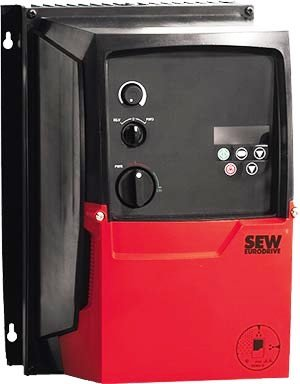
\includegraphics[width=0.70\textwidth]{SEWFU}
\caption{SEW-MCLTEB0022-2A3-4-30}

\begin{itemize}
	\item{Nennleistung: 2,2kW}
	\item{Nennstromspannung: 3x230V}
	\item{Ausgangsnennstrom: 10,5A}
	\item{Schutzart: IP66}
	\item{Preis: 626\textsf{\texteuro}}
\end{itemize}

\end{minipage}
\hspace{0.1\textwidth}
\begin{minipage}[t]{0.45\textwidth}
\framebox[\textwidth]{Frequenzumrichter 2}

%\vspace{-\ht\strutbox}
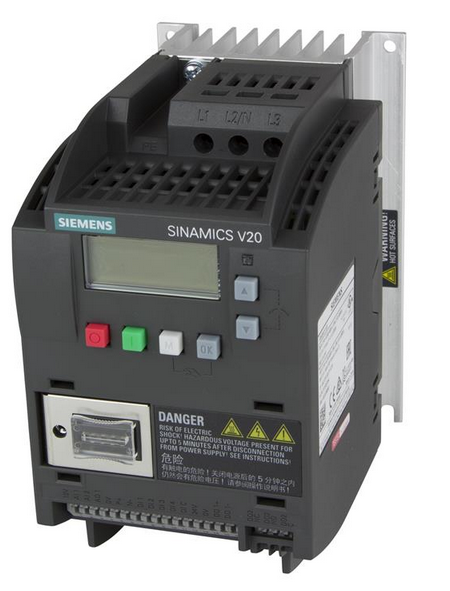
\includegraphics[width=0.68\textwidth]{SiemensV20}
\caption{Siemens-6SL3210-5BE22-2CV0}

\begin{itemize}
	\item{Nennleistung: 2,2kW}
	\item{Nennstromspannung: 3x230V}
	\item{Ausgangsnennstrom: 5,6A}
	\item{Schutzart: IP20}
	\item{Preis: 382,72\textsf{\texteuro}}
\end{itemize}

\end{minipage}
\end{figure}

Die oben genannten Frequenzumrichter erfüllen beide die Anforderungen, um den Motor ansteuern zu können. Aufgrund des niedrigeren Preises wird der Frequenzumrichter zwei von Siemens gewählt. 


%%%%
\newpage
%%%%
\section{Pferderegen}
\label{sec:pferderegen}

Die Wasserversorgung soll dazu dienen, dem Pferd an heißen Sommertagen eine Erfrischung zu ermöglichen. Dafür wird ein Wasseranschluss benötigt. Es gäbe in erster Linie zwei Möglichkeiten, den Wasserfluss zu ermöglichen: Entweder man öffnet manuell ein Wasserhahn, welcher direkt bis zu den Sprühdüsen verbunden ist oder man baut dazwischen ein Magnetventil ein, welches über die App gesteuert werden kann. \\
Prinzipiell ist es Geschmackssache wie man dies haben möchte. In beiden Fällen muss man irgendwo ein Wasserhahn beziehungsweise ein Hauptventil haben, um überhaupt Wasser fließen lassen zu können. 
Mit der Steuerung über die App wird es dem Benutzer ermöglicht, das Hauptventil dauerhaft geöffnet zu lassen. Nur im Winter sollten dafür Vorkehrungsmaßnahmen getroffen werden. Diese werden im Unterkapitel Winterschutz näher erläutert.  

\subsection{Ventil}
\label{sec:ventil}

Die Aufgabe des Ventiles ist einfach: Startet der Benutzer in der App den Sprühregen, gibt das Ventil den Flussweg frei. Man spricht von einem sogenannten Sperrventil. 

\subsubsection{Arbeitsventil}
\label{sec:ventilSuche}

Auf der Suche nach einen geeigneten Ventil für die Bewässerung, ergaben die Suchen meist Ergebnisse für Gartenbewässerungssysteme. In diesen Bereich ganz stark vertreten ist das Unternehmen Gardena. Doch es wurde auch eine Alternative vom Unternehmen Rainbird gefunden. 

\begin{figure}
\begin{minipage}[t]{0.45\textwidth}
\framebox[\textwidth]{Ventil 1}
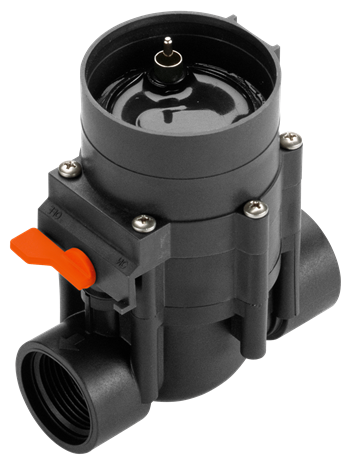
\includegraphics[width=0.7\textwidth]{VentilGardena}
\caption{Gardena 1251-20}

\begin{itemize}
	\item{Betriebsspannung: 9V}
	\item{Art: ?}
	\item{Preis: 68,99\textsf{\texteuro}}
\end{itemize}

\end{minipage}
\hspace{0.1\textwidth}
\begin{minipage}[t]{0.45\textwidth}
\framebox[\textwidth]{Ventil 2}


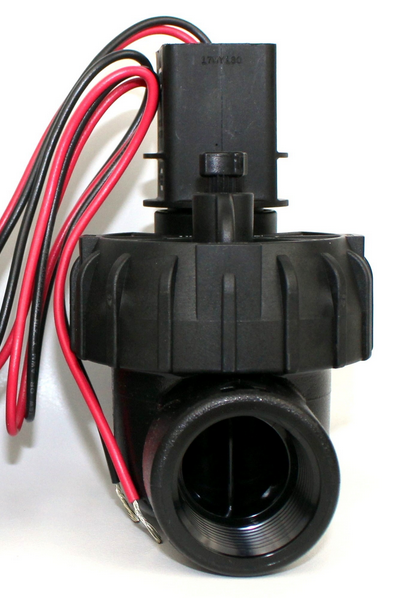
\includegraphics[width=0.63\textwidth]{VentilRainbird}
\caption{BW-MV1-9V}

\begin{itemize}
	\item{Spannung: 9V}
	\item{Art: Impulsventil}
	\item{Preis: 70\textsf{\texteuro}}
\end{itemize}

\end{minipage}
\end{figure} 

Prinzipiell wollen beide Unternehmen, dass man auch das Steuerwerk vom jeweiligen Unternehmen kauft. Deshalb findet man kaum technische Datenblätter dazu und wenn ja, dann dienen diese meist nur der groben Übersicht. Bezüglich den Preis gibt es einen geringen Unterschied von nicht einmal 2 Euro. Bei den Ventil von Pipelife konnte herausgefunden werden, dass es sich um ein 9V-Impulsventil handelt. Wie die Steuerung diesbezüglich aussieht, konnte nicht eruiert werden. Aufgrund dieser Informationen, fiel die Entscheidung auf das 9V-Impulsventil vom Unternehmen Pipelife.

\subsubsection{Funktionstestung Ventil}
\label{sec:funktionstestungVentil}

Um zu überprüfen wie das Ventil wirklich funktioniert, wurde ein Testaufbau gemacht. Dabei wurde mit einen Netzgerät eine Spannung von 9V erzeugt. Damit das Ventil funktioniert, muss ein Wasserdruck vorhanden sein. Aus dem Test wurden folgende Erkenntnisse gewonnen: \\

1.) Das Ventil benötigt zum Betätigen einen Strom von ungefähr 1,72A. \\

2.) Sobald ein positiver Stromimpuls kommt, öffnet sich das Ventil.\\

3.) Das Ventil schließt erst bei fallender Flanke des negativen Impulses.

\subsection{Umpolung}
\label{sec:umpolung}

Aufgrund der oben erworbenen Erkenntnisse, muss bei der Anlage ein Spannungswechsel erfolgen. Dies wird in der Regel mit einer sogenannten H-Brücke realisiert. Die vereinfachte Version lässt sich aus der Abbildung entnehmen. 

\begin{figure}
\begin{center}
	\caption{Vereinfachte H-Brücke}
	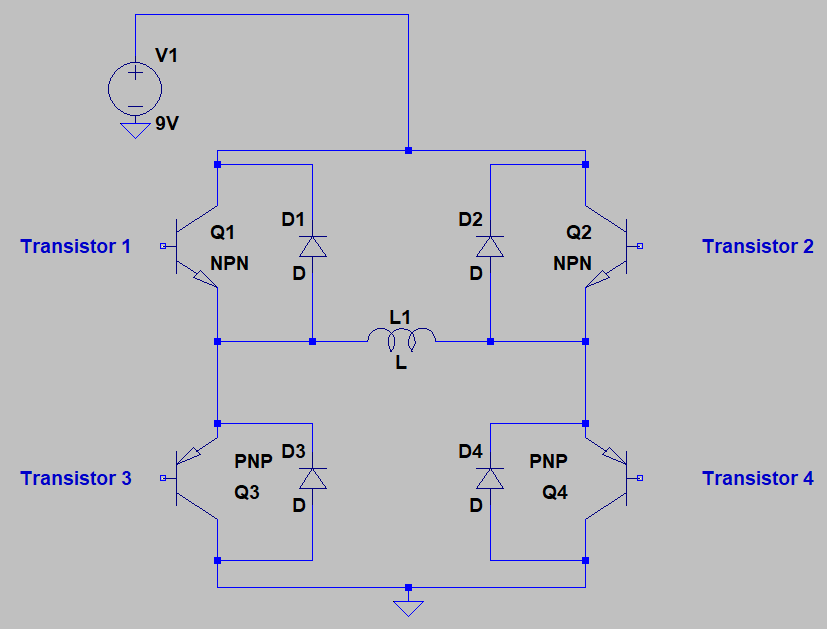
\includegraphics[width=0.6\textwidth]{HBruecke}
\end{center}
\end{figure}

\subsubsection{Funktionsweise}
\label{sec:funktionsweise}

Solange alle Transistoren nicht durchgeschaltet sind, befindet sich der Motor in Ruhezustand. \\
Um das Ventil zu aktivieren, müssen Transistor 1 und Transistor 2 betätigt werden. Daraufhin bekommt das Magnetventil den benötigten Impuls um zu öffnen.\\
Wenn man das Ventil wieder deaktivieren will, müssen die Transistoren 1 und 4 geöffnet werden und danach die Transistoren 2 und 3 geschlossen werden. Nach einer kurzen Verzögerung müssen die Transistoren 2 und 3 wieder geöffnet werden, um das Ventil wieder zu schließen.

\subsubsection{Motortreiber Auswahl}
\label{sec:motortreiberAuswahl}

Auf der Suche nach einer Alternative beziehungsweise einer besseren Variante, wurde die Bausteine VNH2SP30 und der L298 gefunden. Dieser ist ein Motortreiber welcher die H-Brücke bereits integriert hat. Nun gibt es zwei Varianten die Ansteuerung zu realisieren:

\begin{figure}[!ht]
\begin{minipage}[t]{0.45\textwidth}
\framebox[\textwidth]{Variante 1}
\begin{center}
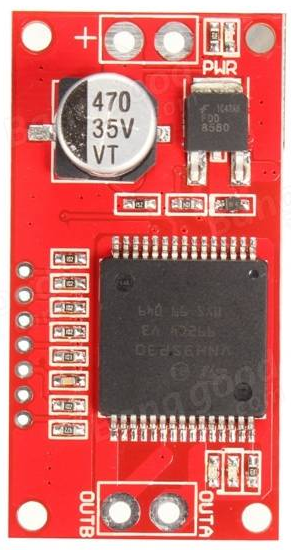
\includegraphics[width=0.4\textwidth]{Motortreiber}
\caption{Single-Chip-VNH2SP30}
\end{center}

\begin{itemize}
	\item{Fertige Beschaltung: Ja}
	\item{Preis: 2,31\textsf{\texteuro}} %https://www.ebay.com/itm/Mini-30A-VNH2SP30-Stepper-Motor-Driver-Monster-Moto-Shield-module-For-Arduino-/331830868475
\end{itemize}

\end{minipage}
\hspace{0.1\textwidth}
\begin{minipage}[t]{0.6\textwidth}
\framebox[\textwidth]{Variante 2}

\begin{center}
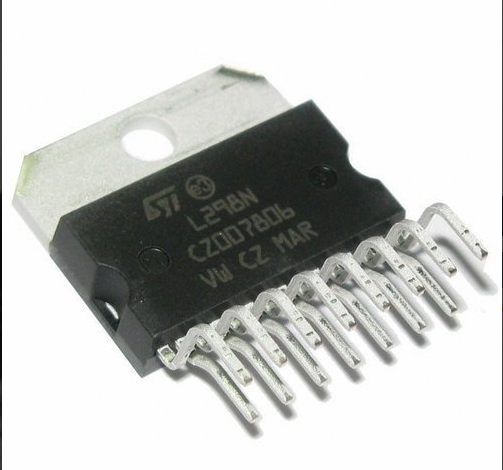
\includegraphics[width=0.64\textwidth]{L298}
\caption{L298}
\end{center}

\begin{itemize}
	\item{Fertige Beschaltung: Nein}
	\item{Preis: 3,79\textsf{\texteuro}} %https://www.conrad.at/de/pmic-voll-halbbrueckentreiber-stmicroelectronics-l298hn-induktiv-bipolar-multiwatt-15-1185128.html
\end{itemize}

\end{minipage}
\end{figure} 

Aufgrund der fertigen Beschaltung und den niedrigeren Preis, wird für die Steuerung des Ventils, der VNH2SP30 den L298 vorgezogen. 

\subsection{Motortreiber Ansteuerung}
\label{sec:motortreiberAnsteuerung}

Der Motortreiber VNH2SP30 hat folgende Pinbelegung:

\begin{itemize}
	\item{Power Supply / Spannungsversorgung / 5V}
	\item{Ground / Masse / GND}
	\item{Enable for motor / Motorfreigabe / CS}
	\item{Clockwise / Im Uhrzeigersinn / INA}
	\item{Counterclockwise / Gegen den Uhrzeigersinn / INB}
	\item{PWM for motor / PWM-Signal für Motor / PMW}
\end{itemize}

Nachfolgend befindet sich ein Beispiel, wie man das Ventil prinzipiell betätigen könnte.

\begin{lstlisting}[language=Arduino]
void setup() {
  pinMode(A0, OUTPUT); //enable 1 // Festlegen der Pinfunktion
  pinMode(7, OUTPUT); //clockwise 1 // Festlegen der Pinfunktion
  pinMode(8, OUTPUT); //counter clockwise 1 // Festlegen der Pinfunktion
  pinMode(5, OUTPUT); //100% PWM 1 // Festlegen der Pinfunktion
  digitalWrite(A0, HIGH);   // enable
  }
void loop() {
  // Positiver Impuls
  digitalWrite(7, HIGH);   // clockwise
  digitalWrite(8, LOW);   // counter clockwise 
  digitalWrite(5, HIGH);   // 100% PWM
  delay(5000);              // wait for a second
  // Negativer Impuls
  digitalWrite(7, LOW);   // clockwise
  digitalWrite(8, HIGH);   // counter clockwise 
  digitalWrite(5, HIGH);   // 100% PWM 
  // Flanke fallen lassen
  digitalWrite(7, LOW);   // clockwise
  digitalWrite(8, LOW);   // counter clockwise 
  digitalWrite(5, HIGH);   // 100% PWM
  delay(5000);              // wait for a second
}
\end{lstlisting}

In diesen Programmablauf würde das Ventil ständig wechseln, zwischen den Zuständen offen und geschlossen. Das PWM-Signal wird mit 100 Prozent, da das Ventil nur geöffnet oder geschlossen sein kann. Halb offen gibt es nicht. \\
Für die Realisierung in der Anlage gibt es zwei Möglichkeiten: ein Software- beziehungsweise ein Hardwareevent muss eintreten, damit das Ventil sich öffnen oder schließen soll. Da die Anlage über die App gesteuert werden soll, muss die Abfrage über Softwareevent erfolgen. Dies wird mittels Interrupt gelöst. Ein Interrupt ist eine Unterbrechung im Programm. Dieser beendet kurzzeitig das Programm, führt die Interrupt Service Routine aus, und setzt danach an der zuvor unterbrochenen Stelle fort. \\ In der Interrupt Service Routine, bekommt eine globale Variable den jeweiligen gewünschten Zustand, ob die Pferdekühlung aktiviert werden soll oder nicht. Im Hauptprogramm wird die globale in der lokalen Variable geschrieben. Mittels einer Doppelverzweigung wird als erstes entschieden, ob das Ventil geöffnet werden soll. Die nächste Abfrage überprüft, wie lange der Sprühregen aktiviert ist. Sollte er länger  Dort werden im jeweiligen Fall die gewünschten Pins betätigt.

\subsection{Wasserversorgung}
\label{sec:wasserversorgung}

Um überhaupt die Anlage mit Wasser versorgen zu können, muss ein Wasseranschluss vorhanden sein. Von dort muss das Wasser zum Ventil zugeführt werden und anschließend aufgeteilt werden. Welchen Durchmesser der Wasseranschluss hat. Diese sind im Normalfall in Zoll angeben und haben entweder 1/2, 3/4 oder 1 Zoll. Um keinen hohen Druckverlust zu bekommen, wird ein Rohrsystem mit einem Innendurchmesser von 3/4 Zoll festgelegt. Das heißt sollte das System keine 3/4 Zoll haben, muss mit Verbindungssystemen umgewandelt werden. Es sollten so wenig Verbindungsstücke wie möglich verwendet werden, um unnötige Druckverluste zu vermeiden. Der idealste Fall wäre in diesen Fall ein 1 Zoll Anschluss. \\ 


\subsubsection{PE-Rohr}
\label{sec:peRohr}

Nach sorgfältiger Recherche wurde folgende PE-Rohre gefunden:\\

\begin{figure}
\begin{center}
	\caption{PE-Rohr}
	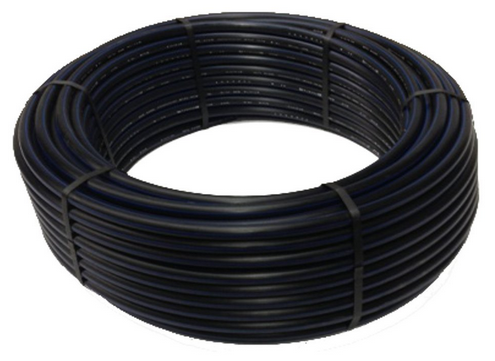
\includegraphics[width=0.3\textwidth]{PEROHR}
\end{center}
\end{figure}

Diesen Schlauch gibt es von diesem Unternehmen in folgenden 3 Varianten:

\begin{itemize}
	\item{1/2 Zoll // Preis: 0,70\textsf{\texteuro} pro Meter}
	\item{3/4 Zoll // Preis: 0,90\textsf{\texteuro} pro Meter}
	\item{1 Zoll // Preis: 1,20\textsf{\texteuro} pro Meter}
\end{itemize}

Diese erfüllen folgende Eigenschaften:

\begin{itemize}
	\item{Maximal Betriebsdruck: 12,5 bar}
	\item{Durchmesser: 1 Zoll}
	\item{Für Trinkwassergebrauch zugelassen}
	\item{Flexibel bei Verlegung}
	\item{100 Jahre Lebensdauer}
\end{itemize}


Je nachdem wie weit der Wasseranschluss von der Pferdeführanlage entfernt ist wird der Rohrweg größer. 

\subsubsection{Ventilübergang}
\label{sec:ventiluebergang}

Um den Schlauch mit dem Ventil zu verbinden, wird ein Übergangsstück benötigt, welches ein Gewinde mit dem Schlauchende verbinden soll. Dafür wurde folgende Verbindung gefunden:

%https://www.amazon.de/GARDENA-Sprinklersystem-Verbinder-Bew%C3%A4sserungsventile-Verbindungstechnik/dp/B000OY2KSW/ref=sr_1_4?ie=UTF8&qid=1520768397&sr=8-4&keywords=1+zoll+verbinder (11.3.2018)

\begin{figure}
\begin{minipage}[t]{0.45\textwidth}
\framebox[\textwidth]{Variante 1 (1 Zoll)}
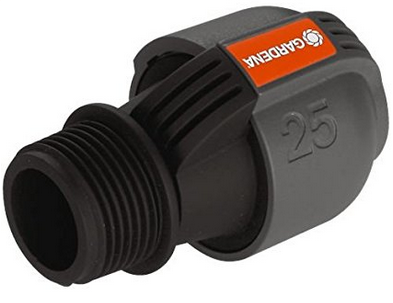
\includegraphics[width=0.7\textwidth]{GardenaVerbindung}
\caption{Gardena Verbindungsstück}

\begin{itemize}
	\item{Preis: 3,55 \textsf{\texteuro}}
	\item{Gewinde: 1 Zoll}
	\item{Schlauchdurchmesser: 1 Zoll}
\end{itemize}
\end{minipage}
\hspace{0.1\textwidth}
\begin{minipage}[t]{0.45\textwidth}
\framebox[\textwidth]{Variante 2 (3/4 Zoll)}


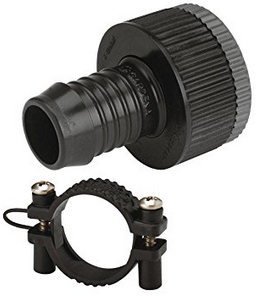
\includegraphics[width=0.63\textwidth]{Gardena1auf34}
\caption{Gardena Übergang}

\begin{itemize}
	\item{Preis: 4,89 \textsf{\texteuro}}
	\item{Gewinde: 1 Zoll}
	\item{Schlauchdurchmesser: 3/4 Zoll}
\end{itemize}

\end{minipage}
\end{figure} 

Da nun der Anschluss des Ventiles ermöglicht wurde, muss nun die Versorgung für die Sprühdüsen erstellt werden. 

Der Innenzaunradius beträgt 8,75 Meter. Daraus ergibt sich ein Umfang von zirka 55 Meter. Es werden 8 Sprühdüsen, mit 45 Grad Abstand, aufgestellt. Nun muss 



\newpage

\subsubsection{Sprühnebel Erzeugung}
\label{sec:spruehnebel}

%https://www.amazon.de/BQLZR-Kunststoff-Nebeld%C3%BCse-Spr%C3%BChkopf-Bew%C3%A4sserungsszstem/dp/B00QUUGAQC/ref=sr_1_3?ie=UTF8&qid=1520697676&sr=8-3&keywords=nebeld%C3%BCse ( 11.3.2018)





%%%%
\newpage
%%%%
\section{Geschwindigkeitsmessung}
\label{sec:geschwindigkeitsmessung}
%%%%
\newpage
%%%%
\section{Kommunikationsschnittstelle}
\label{sec:kommunikationsschnittstelle}
%%%%
\newpage
%%%%
\section{Sicherheit der Pferde und Anlage}
\label{sec:sicherheitDerPferdeUndAnlage}

\subsection{Allgemeine Sicherheitsfragen}
\label{sec:allgemeineSicherheitsfragen}

Um die Anlage bei Tieren aktivieren zu können, muss man auch eine Basissicherheit gewährleisten.
Diesen Bereich darf man nicht vernachlässigen. \\ In Folgenden Abschnitt  kann in manchen Fällen nicht zwischen Besitzer oder Eigentümer Rücksicht genommen werden , da es beide Fälle in der Praxis geben kann. Deshalb bleibt primär der Eigentümer für die Wartungen und den Anlagenschutz haftbar. Sollte der Eigentümer die Anlage in der Regel nicht verwenden, kann er die jeweiligen Wartungs--- und Sicherheitsaufgaben auf den Besitzer übertragen. Dieses muss aber in schriftlicher Form erfolgen. In diesen Fall muss der Besitzer im nachfolgenden Kontext die Aufgaben des Eigentümers erfüllen.

Bei unserer Pferdeführanlage können folgende Fehler bewusst auftreten:

\begin{itemize}
\item{Was passiert, wenn ein Pferd hinfällt?}
\item{Was passiert wenn ein Pferd stur stehen bleibt?}
\item{Was passiert wenn das Pferd die Anlage anschieben will (schneller ist)?}
\item{Was passiert wenn die Anlage nicht arbeitet wie gewünscht?}
\item{Welche Vorkehrungen gibt es im Bereich Blitzschutz?}
\end{itemize}

\subsection{Tierschutzgesetz und Anlagenschutz}
\label{sec:tierschutzgesetzUndAnlagenschutz}

Gemäß §5 Abs. 1 Tierschutzgesetz ist es verboten, 
einem Tier ungerechtfertigt Schmerzen, Leiden oder Schäden zuzufügen oder es in schwere Angst zu versetzten. 
Unter §5 Abs. 2 Satz 3 lit. b wird nochmals extra darauf hingewiesen, dass keine technischen Geräte verwendet werden, welche das Verhalten eines Tieres durch Härte oder durch Strafreize zu beeinflussen. 

Somit darf man dem Ross mit unserer Anlage, keine kleinen Denkimpulse geben, wenn es stur stehen bleibt. Wenn das Reitvieh stehen bleibt, darf ihm und der Anlage selbst nichts passieren. Die einfachste und sicherste Lösung ist, die Anlage zu stoppen. Wenn die Anlage weiter fahren möchte, könnten ungewollte Momente auftreten und somit mechanische Schäden in der Anlage verursachen.

Folgende Vorkehrungen wurden auf der elektrischen Seite zum beidseitigem Schutz getroffen:

Sobald die Auswertung des Sensors merkt, dass die Anlage unfreiwillig stehen bleibt, schaltet die Anlage automatisch ab. Daraufhin muss der jeweilige Eigentümer überprüfen, ob es ein technischer Fehler oder ein Problem beim Pferd vorliegt, bevor er diese wieder in Betrieb nimmt
Die Gitter, hinter beziehungsweise vor dem Pferd, werden zum Schutz des Tieres nicht elektrisch verbunden.
Welcher Zaun neben den Gitter gebaut wird, bleibt dem Eigentümer selbst überlassen.

Sollte man einen Elektrozaun beziehungsweise doch Strom durch die Gitter schicken, werden die Pferde in der Anfangsphase leicht gestresst sein. Sobald sie sich daran gewöhnt haben, funktioniert er wie ein normaler Zaun und die Pferde wissen, dass sie diesen nicht berühren sollten.
Bei den Gittern mit Strom würden die Pferde sogar mehr geschützt werden, wenn sie mit Strom durchflossen werden. Grund dafür ist, dass sich die Pferde an den Stangen Verletzungen zu ziehen könnten, als mit kurzen Stromimpulsen. In Österreich ist dies aber nicht gesetzeskonform.

\subsection{Blitzschutz}
\label{sec:blitzschutz}

Da unsere Pferdeführanlage im Freien steht, darf man auch den Fall eines Blitzeinschlags nicht vernachlässigen. 
Die Durchschnittsanzahl von Blitzen in Österreich wird mit zirka 5 Blitze pro 1km\textsuperscript{2} in einem Jahr geschätzt. 
Die Anlage darf nicht in Betrieb genommen werden, wenn der Betreiber bemerkt, 
dass es in wenigen Minuten ein Gewitter geben könnte.
Sollte die Anlage während eines Gewitters in Betrieb genommen werden, 
gibt es ein erhöhtes Risiko für die Pferde und der Anlage selbst.
Die Haftung liegt in diesem Fall bei der Person, die die Anlage in dieser Zeit in Betrieb nimmt.

\subsection{Winterschutz}
\label{sec:winterschutz}

Die Zeit, in der Winterschutz unserer Pferdeführanlage in Kraft tritt, ist die gleiche wie die Winterreifenpflicht in Österreich. Das heißt vom 1. November bis 15. April muss die Anlage winterfest gemacht sein. 
\\
\\
In folgenden Bereichen muss ein Winterschutz vorgenommen werden:
\begin{description}
\item[Boden:]
Den Untergrund wo sich die Pferde bewegen muss der Eigentümer selbst wählen. Bei Temperaturen unter 6 Grad Celsius, darf der Sprühregen nicht mehr aktiviert werden. Nachdem das Wasser gefroren ist kann das Reitvieh am glatten Boden ausrutschen und gleichzeitig könnte es zu Komplikationen der Pferdeführanlage selbst kommen. Hierfür ist die jeweilige Person haftbar, die das Drehsystem in Betrieb genommen hat.

\item[Wasserrohre:]

Um ein langes Leben der Wasserrohre gewährleisten zu können, muss der jeweilige Eigentümer vor den jährlich wiederkommenden Kälteperioden das Wasser aus den Rohren entfernen. Eine der gängigsten Methoden ist es, das Wasser in den Wasserleitungen durch ein kleines Entwässerungsventil zu entleeren. Das elektromagnetische Ventil muss manuell geöffnet werden, damit das Wasser zu rinnen beginnt. Wäre das Ventil geschlossen, könnte das Wasser nicht fließen, da ein Unterdruck in der Leitung erzeugt werden würde. Mittels Druckluft kann auch das restliche Wasser ausgeblasen werden. Somit sind die Wasserrohre für den Winter gerüstet.

\end{description}

\subsection{Redundanz}
\label{sec:redundanz}

Im Bereich Sicherheit von Anlagen, kann man häufig den Begriff Redundanz aufschnappen. 

 Redundanz (lat. = Überfluss) ist das Vorhandensein zusätzlicher technischer Komponenten, die für den Betrieb eines Systems oder Gerätes nicht nötig sind, solange keine Störung bzw. kein Ausfall vorliegt. \footnote{http://www.secupedia.info/wiki/Redundanz}

Sollte die Pferdeführanlage vermarktet werden, könnte man die Anlage erweitern. Diese Erweiterung betrifft den Bereich für die Sicherheit der Pferde.

\begin{center}
	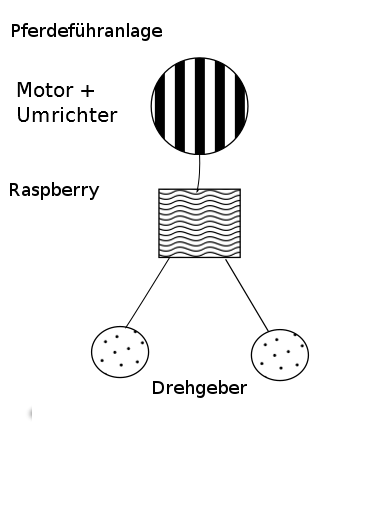
\includegraphics[width=0.5\textwidth]{Redundanz}
\end{center}

Das Bild zeigt eine Möglichkeit die Redundanz zu realisieren.

Gedanke dabei ist, wenn ein Drehgeber defekt ist, kann auch noch der zweite Inkrementalgeber ein Signal liefern, um zumindest einen Durchlaufzyklus beenden zu können. Die hängt aber davon ab, ob der jeweilige Benutzer überhaupt möchte ob es die Anlage weiterlaufen soll und ob er dafür zusätzlich zahlen möchte. Somit könnte man ein Sicherheitsextra zusätzlich anbieten.

Natürlich gibt es auch noch andere Varianten, das System redundant zu machen. Doch dies wäre eine zusätzliche 
